\subsection{SP-18 (OSY)}
Virtualizace hlavní paměti stránkováním, principy překladu virtuálních adres na fyzické, struktura tabulek stránek, algoritmy pro nahrazování stránek.

\textbf{Princip virtuální paměti se stránkováním:}
\begin{itemize}
	\item Proces používá virtuální/logické adresy, ty adresují virtuální adresní prostor
	\item VAS (virtual adress space) je rozdělen na stejně velké stránky --- typicky 4KB nebo 8KB
	\item na stejně velké úseky (rámce) je rozdělena fyzická paměť
	\item aktuálně používané stránky musí být aktuálně v hlavní paměti 
	\item virtuální adresa = číslo stránky + offset
\end{itemize}

\textbf{Možnosti překladu adres:}
\begin{itemize}
	\item jednoúrovňová tabulka stránek
	\item víceúrovňová tabulka stránek
	\item invertovaná tabulka stránek
\end{itemize}

Překlad adres zajišťuje MMU s TLB (viz \ref{OB-6}).

\textbf{Jednoúrovňová TS:}
\begin{itemize}
	\item pro každou stránku VAS daného procesu obsahuje jeden řádek obsahující číslo rámce a kontrolní bity (Present bit (P) --- je stránka v hlavní paměti?, Reference bit (R) --- přistupovalo se ke stránce?, Modify bit (M) --- byl obsah modifikován?, Přístupová práva, Cache disabled/enabled, R/W, User/Supervisor (U/S) - lze přistupovat v uživatelském módu?)
	\item číslo stránky = index do této tabulky
	\item pro každý proces jedna tabulka
\end{itemize}

\textbf{Víceúrovňová TS:}
\begin{itemize}
	\item virtuální adresa se skládá z $n$ indexů, které ukazují do tabulek jednotlivých úrovní + offset
	\item tabulky stránek úrovní 1,...,$n-1$ obsahují číslo rámce kde je následující tabulka + present bit
	\item tabulka úrovně $n$ obsahuje present bit + číslo rámce hledané stránky
	\item hlavní/první tabulka je v paměti vždy
\end{itemize}

\textbf{Invertovaná TS:}
\begin{itemize}
	\item obsahuje pro každý rámec fyzické paměti jeden řádek, kde je uloženo: číslo stránky nahrané do rámce, číslo procesu, kterému stránka patří, kontrolní bity, index zřetězení (stejně velký jako index do tabulky)
	\item existuje 1 tabulka pro celý systém
	\item číslo stránky se hashovací funkcí převede na index do tabulky
	\item více stránek se může namapovat na stejný rámec --- proto index zřetězení
\end{itemize}

\newpage
Řešení výpadku stránek:

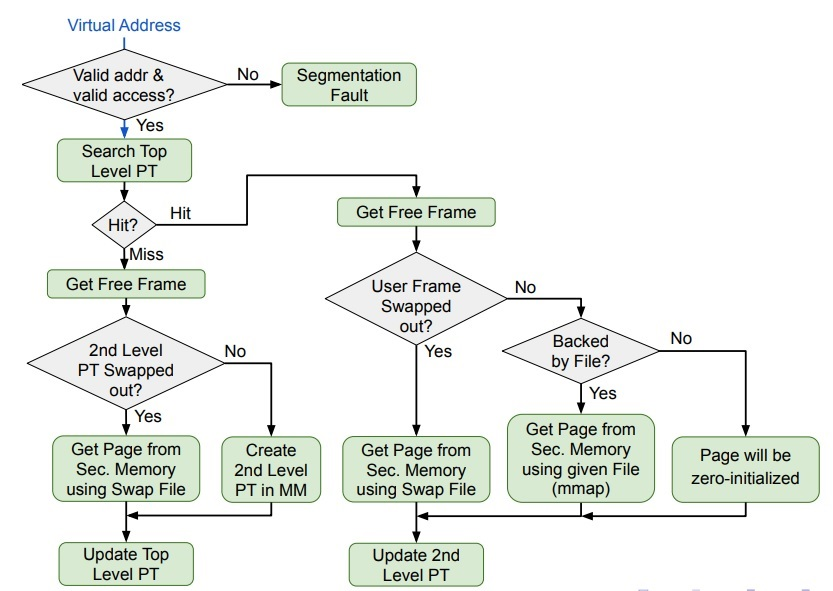
\includegraphics[width=0.6\textwidth]{img/SP-18_0.jpg}
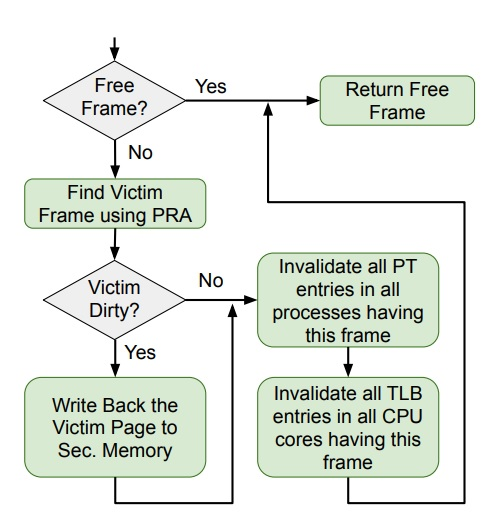
\includegraphics[width=0.35\textwidth]{img/SP-18_1.jpg}

\subsubsection*{Algoritmy pro náhradu stránek}
V okamžiku kdy většina/všechny rámce fyzické (hlavní) paměti jsou obsazené, je úkolem OS najít vhodný rámec, jehož obsah (stránka) se uvolní. K tomu slouží algoritmy pro náhradu stránek.

\textbf{Co je od takových algoritmů požadováno?}
\begin{itemize}
	\item minimalizace počtu výpadků stránek
	\item rychlost
	\item jednoduchá implementace
\end{itemize}

Tyto algoritmy využívají proncipů prostorové a časové lokality.

\textbf{Optimální algoritmus:}
\begin{itemize}
	\item nahradí se stránka, která má čas příštího přístupu nejdelší
	\item generuje minimální počet výpadků stránek
	\item sice nelze udělat, ale slouží pro porovnání kvality reálných algoritmů
\end{itemize}

\textbf{NRU (Not Recently Used)}
\begin{itemize}
	\item pro každou stránku se pamatuje reference bit (R) a modified bit (M) (viz výše)
	\item reference bit se periodicky nastavuje na 0
	\item stránky jsou rozděleny do 4 tříd (RM == 00, RM == 01, RM == 10, RM == 11)
	\item nahradí se nějaká stránka z co nejnižší třídy (tedy 00 $\rightarrow$ 01 $\rightarrow$ 10 $\rightarrow$ 11)
\end{itemize}

Jednoduchý na pochopení i implementaci, poměrně nízký počet výpadků stránek.

\textbf{FIFO (First In First Out)}
\begin{itemize}
	\item je udržován seznam stránek nahraných v paměti
	\item nově nahraná stránka je zaznamenána na konec seznamu
	\item nahrazena je první stránka ze seznamu
\end{itemize}

Jednoduchý na pochopení i implementaci, ale generuje poměrně vysoký počet výpadků stránek.

\textbf{Clock algoritmus}
\begin{itemize}
	\item modifikovaný FIFO algoritmus
	\item seznam stránek jako kruhová fronta
	\item na počátku ručička ukazuje na první položku seznamu
	\item pro každou položku je zaznamenán reference bit, který je nastaven na 1 při pridání stránky do seznamu a při přístupu k ní
	\item při potřebě náhrady stránky ručička u položky, na kterou ukazuje, zjistí stav R bitu --- pokud 1, vynuluje a jde na další položku --- pokud 0, tato stránka se nahradí a ručička se posune
\end{itemize}

Jednoduchý na implementaci, generuje poměrně nízký počet výpadků stránek. Existují varianty s více ručičkami, kde podle rychlosti posunu ručiček a jejich rozevření je definováno časové okno, dle kterého zjišťujeme, zda byla stránka nedávno použita.

\textbf{LRU (Least Recently Used)}
\begin{itemize}
	\item vybere se stránka, která je nejdelší dobu bez přístupu
	\item pro každou položku je navíc zapamatován čas použití, který se aktualizuje při každém použití (existuje globální čítač, který se zvýší při každém přístupu do paměti, jeho hodnota je pak zanesena k právě použité stránce)
	\item kandidát je taková stránka, která má nejnižší čas posledního přístupu (nutno porovnat všechny)
\end{itemize}

Generuje poměrně nízký počet výpadků stránek, dobrá aproximace optimálního algoritmu. Složitější implementace (čítač s časem a porovnání všech stránek)

\textbf{Aging algoritmus}
\begin{itemize}
	\item simulace LRU lgoritmu
	\item pro každou stránku je zapamatováno: R bit (nastaví se na 1 při každém přístupu), $n$-bitový čítač \textit{C}, který má po načtení stránky do paměti všechny bity na 1
	\item periodicky se pro každou stránku \textit{C} posune o 1 doprava, jeho nejvýznamější bit se nastaví na R, a R se nastaví na 0
	\item vhodným kandidátem je stránka s nejnižší hodnotou \textit{C}
\end{itemize}

Menší režie než LRU, ale není tak přesný (nepamatuje se přesný čas, ale jen interval, kdy se naposledy přistupovalo --- omezená historie).